\documentclass[twocolumn]{revtex4}

\usepackage{graphicx,amsmath}

\newcommand{\bra}[1]{\left< #1 \right|}
\newcommand{\ket}[1]{\left| #1 \right>}
\newcommand{\braket}[2]{\left< #1 | #2 \right>}
\newcommand{\innerp}[3]{\left< #1 | #2 | #3 \right>}

\newcommand{\figwidth}{0.33\textwidth}

\hyphenation{transmon}

\begin{document}

\title{Artificial Atoms: Modeling the Inductively-Shunted Cooper Pair
  Box}
\author{John O'Connor, Jens Koch, Steven Girvin, Vlad Manucharyan, Lev
  Bishop, Schoelkopf et al, Devoret et al}

\begin{abstract}
  The Cooper pair box (CPB) is a well-studied quantum circuit that can be
  function as an artificial atom. The inductively-shunted Cooper pair
  box (CPBL) is much less well-studied. Adding an inductive shunt
  promises to mitigate ambient charge noise around the circuit, but it
  also produces a Hamiltonian with completely different
  characteristics. The first examples of these circuits are being
  studied in by Vlad Manucharyan, and while computer models of the
  energy spectrum for these circuits exist, they are too slow to be
  helpful in interpreting the experimental data. We develop a more
  efficient model that is fast enough to run curve fitting on
  experimental data, and demonstrate the results of this model.
\end{abstract}

\maketitle

\section{Introduction}

Quantum computing offers a number of enticing theoretical speedups
over classical computers. Best known is Peter Shor's factoring
algorithm, which can factor large composite numbers in polynomial
time. This has the potential to break popular cryptographic schemes
like RSA that rely on the intractability of the factoring
problem. Another less dramatic but more widely applicable speedup is
Grover's algorithm for searching an arbitrary space of $n$ elements in
time $O(n)$, a quadratic improvement over the classical case. These
and other quantum algorithms have motivated significant research in
the field of quantum computing.

The greatest obstacle to constructing a quantum computer has been to
create the quantum bits (qubits) that store information in
superposition. Any quantum system tends to decohere due to
interactions with its environment, and a qubit has to meet two
contradictory requirements. First, it must be sufficiently decoupled
from its environment to hold its state long enough to perform
meaningful computation. At the same time, though, it has to be coupled
to its environment enough to be reliably measurable with the
computation is finished. This is difficult enough that, at present,
one of the largest quantum computations ever performed
\cite{Vandersypen} was the factorization of the number $15$.

One of the fields in which research is proceeding on this front is
circuit quantum electrodynamics. Quantum circuits have several
potential advantages over other forms of qubits. They sit on a chip
rather than migrating through space, which greatly simplifies research
compared to various atomic methods, and they can be manufactured using
fairly standard circuit printing techniques. More importantly, while
atomic systems have fixed energy spectra, researchers can tune the
parameters of their quantum circuits to produce artificial atoms with
a range of different spectra.

Computer models of these circuits can aid experimental research in
several ways. Theoretical models of the device spectrum highlight
extraneous or unexpected features in the data, and help in identifying
those features. Computer models can explore parameter regimes not yet
probed by experiment, in seconds rather than weeks. Also, in our case
at least, the manufacturing processes for our circuits involve
significant uncertainties. Insulating layers in a Josephson junction,
for example, are created by depositing a layer of aluminum, allowing
it to oxidize for a period of time, and depositing a second aluminum
layer on top. The thickness of the resulting oxide layer is highly
variable, and it continues to grow after the circuit is already
complete. For this and similar reasons, the design parameters of our
circuits are unknown until we measure them against theoretical models.

\section{Modeling the Cooper Pair Box}

\begin{figure}
  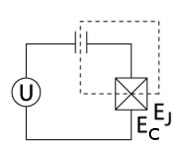
\includegraphics[width=\figwidth]{CPB-circuit.png}
  \caption{A diagram of the Cooper Pair Box. Note that $E_C$ and $E_J$
    are both parameters of the Josephson junction.}
  \label{cpb-circuit}
\end{figure}

One well-studied example of a quantum circuit is the Cooper Pair Box
(CPB). See Fig.~\ref{cpb-circuit}. We used the basic CPB as an initial
test of our modeling techniques, and we use it here as an introduction
to the inductively-shunted Cooper pair box (CPBL). The CPB is a
superconducting circuit with three components: a voltage source, a
gate capacitor, and a Josephson junction.

\begin{figure}
  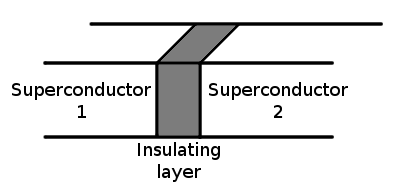
\includegraphics[width=\figwidth]{junction.png}
  \caption{ A Josephson junction }
  \label{junction}
\end{figure}

A Josephson junction (Fig.~\ref{junction}) is a circuit element
consists of two superconducting leads joined across a thin insulating
boundary. In our devices, Josephson junctions are constructed by
depositing a layer of aluminum, allowing a thin oxide layer to form on
the surface of that layer, and finally depositing a second layer of
aluminum on top. The oxide acts as an insulator, and at sufficiently
low temperatures the aluminum leads become superconducting. A
Josephson junction acts like a capacitor across its insulating layer,
but it also allows Cooper pairs of electrons to tunnel through. We can
treat the Josephson junction as a capacitor and a tunneling junction
in parallel, and we denote the capacitance and tunneling coefficient
of these virtual components by $E_C$ and $E_J$, respectively.

The capacitative properties of the Josephson junction, together with
the gate capacitor, create a superconducting island in the CPB,
indicated by the dotted line in Fig.~\ref{cpb-circuit}. This lets us
treat the CPB in its ``charge basis,'' where each eigenstate denotes a
number of Cooper pairs added to or removed from the island. In the
charge basis, the Hamiltonian of the CPB is
\begin{align}
\label{cpb-H}
\begin{split}
  H_{\text{CPB}} = \sum_{n=-\infty}^{+\infty}& \frac{-E_J}{2}\left(
      \ket{n}\bra{n-1} + \ket{n-1}\bra{n} \right) \\
    & {} + 4E_C(n-N_g)^2\ket{n}\bra{n},
\end{split}
\end{align}
where $n$ represents the number of tunneled electron pairs and $N_g$
is the offset charge across the capacitor.

In order to calculate the energy spectrum of the CPB as a function of
the offset charge, $N_g$, we will need to express that Hamiltonian as
a matrix in the charge basis. Note that $H_{\text{CPB}}$ will be an
infinite matrix not just downward and rightward but, because $n$ and
$m$ can take all integer values, leftward and upward as well. Each
matrix element ${H_{\text{CPB}}}_{nm}$ is equal to the inner product
$\innerp{n}{H_{\text{CPB}}}{m}$, and so specifying the matrix only
requires specifying those products. Eqn.~\ref{cpb-H} gives us:
\begin{equation}
  \innerp{n}{H_{\text{CPB}}}{m} = \left\{\begin{array}{lcl}
        4E_C(n-N_g)^2 & : &n=m \\
        \frac{-E_J}{2} & : &|n-m|=1\\
        0 & : & \text{otherwise}
        \end{array}\right.
\end{equation}

Truncating this tridiagonal matrix allows us to approximate its
eigenvalues numerically. The eigenvalues depend only on the ratio
between $E_J$ and $E_C$, and we can plot the energy spectra relative
to $N_g$ for several values of this ratio in Figures \ref{cpb-1},
\ref{cpb-10}, and \ref{cpb-30}. Units on the y-axis are in
gigahertz. We can see that for values where $E_J$ is dominant
(Fig.~\ref{cpb-1}) the spectrum looks like a series of parabolas,
which results from the quadratic term on the diagonal of
$H_{\text{CPB}}$. For larger values the spectral lines smooth out and
move apart, approaching a constant spacing.

\begin{figure}
  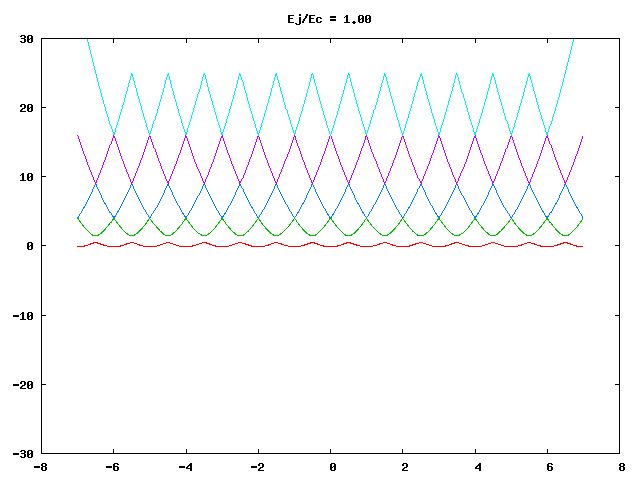
\includegraphics[width=\figwidth]{CPB-1.png}
  \caption{Energy spectrum vs. $N_g$ for the CPB with
    $\frac{E_J}{E_c}=1$}
  \label{cpb-1}
\end{figure}
\begin{figure}
  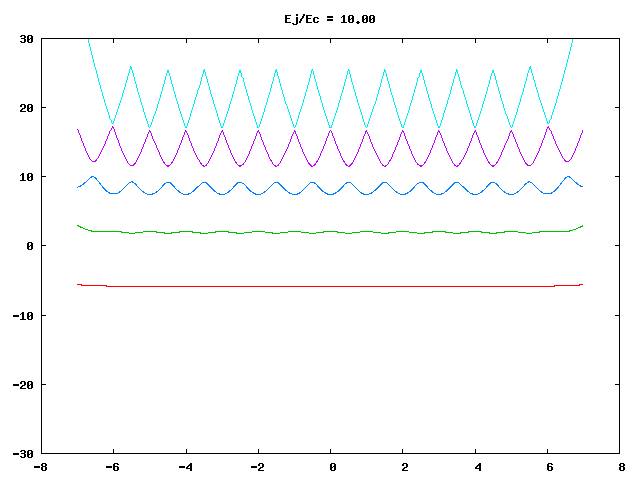
\includegraphics[width=\figwidth]{CPB-10.png}
  \caption{Energy spectrum vs. $N_g$ for the CPB with
    $\frac{E_J}{E_c}=10$}
  \label{cpb-10}
\end{figure}
\begin{figure}
  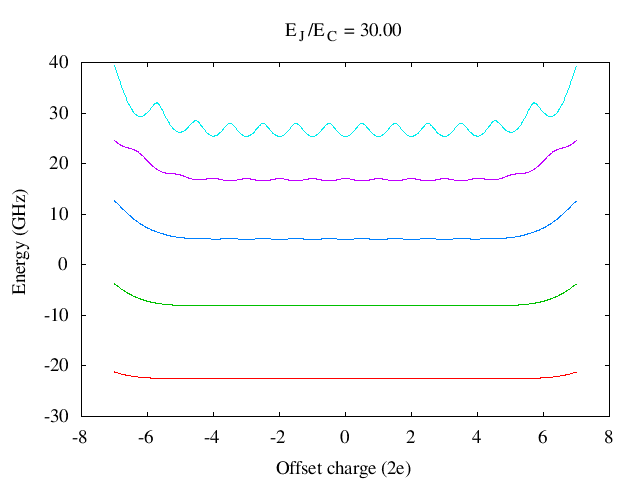
\includegraphics[width=\figwidth]{CPB-30.png}
  \caption{Energy spectrum vs. $N_g$ for the CPB with
    $\frac{E_J}{E_c}=30$. Note that the divergences on the left and
    right ends of each line are an artifact of the approximation
    process, not of the theory itself. Extending the matrix cutoff
    pushes these divergences farther out in $N_g$.}
  \label{cpb-30}
\end{figure}

\section{Challenges with the CPB}
As with all quantum circuits, one of the primary goals is to lengthen
the time before decoherence. In the case of the CPB, one of the
primary causes of decoherence is the charge noise---slow, randomly
oscillating charges in the environment that introduce noise into the
offset charge, $N_g$.

Several strategies exist for mitigating the effects of charge noise in
the CPB. One approach is to operate the device near local extrema of
the energy spectrum. We can see in Fig.~\ref{cpb-1} that at certain
values of $N_g$ all of the spectral lines of the CPB reach local
maxima or minima. In particular for that figure, the maxima of the
ground level and the minima of the first excited state are both fairly
smooth. When the CPB is operated at these points, the first order
effects of charge noise drop out, though this technique is limited by
the precision of $N_g$.

Another approach is to operate the CPB in the ``transmon'' region
where $EJ\ll EC$. We can see in Fig.~\ref{cpb-30} that the spectral
lines become very flat, reducing the effects of charge noise even
further. One of the difficulties of working in the transmon region is
that, as we mentioned earlier, the spacing between spectral lines
becomes uniform. This makes the energy differences between states
small integer multiples of one another. Because a qubit generally
needs to be restricted to two energy states, this accessibility of the
higher states can be a substantial problem.

\begin{figure}
  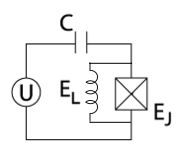
\includegraphics[width=\figwidth]{CPBL-circuit.png}
  \caption{ A diagram of the inductively shunted Cooper pair box
    (CPBL). The circuit now has three parameters, $E_C$ and $E_J$
    associated with the Josephson junction, and $E_L$ associated with
    the inductor.}
  \label{CPBL-circuit}
\end{figure}

A third option---the option that we explore here---is to add an
inductive shunt to the CPB (Fig.~\ref{CPBL-circuit}). The energy
spectrum of the CPBL is entirely distinct from that of the CPB and
worthy of study in its own right, but it is also much less sensitive
to charge noise. This results from the fact that at low
frequencies---that is, at the frequencies of charge noise---the
inductor acts like a closed circuit and shunts those signals
aside, while at high frequencies---like those of our input
voltages---the inductor approximates an open circuit, and the CPBL
behaves similarly to the CPB.

\section{Modeling the Inductively Shunted Cooper Pair Box}

Adding the inductor requires that we make several changes to our
equations. First, since no superconducting island exists in the CPBL,
the charge basis is no longer meaningful. We will instead use another
basis from the CPB called the phase basis. The phase term arises from
the Josephson equations, which we do not derive here. (See
\cite{Feynman}.) Expressed in the phase basis, the Hamiltonian of the
CPB takes the form
\begin{equation}
  H_{\text{CPB}} = -4E_C\frac{d^2}{d\varphi^2}-E_J\cos{\varphi},
\end{equation}
where $\varphi$ varies from $0$ to $2\pi$.

Another consequence of the missing island is that no offset charge can
exist on the CPBL, and so we will instead plot the energy spectrum
with respect to $\phi$, the magnetic flux through our inductor. The
$\phi$ parameter comes into the picture when we add the term for our
inductor to $H_{\text{CPB}}$, producing the Hamiltonian
\begin{equation}
  H = -4E_C\frac{d^2}{d\varphi^2}-E_J\cos{\varphi}+\frac{1}{2}
  E_L\left(\varphi-\frac{2\pi\phi}{\phi_0} \right)^2.
\end{equation}
This equation also introduces a third design parameter for the CPBL,
the strength of the inductor, $E_L$. In order to analyze this
equation, we will immediately adopt a change of variables, $\varphi
\rightarrow (\varphi + \frac{2\pi\phi}{\phi_0})$:
\begin{equation}
  H = -4E_C\frac{d^2}{d\varphi^2}-E_J\cos\left(\varphi+
    \frac{2\pi\phi}{\phi_0}\right)+
  \frac{1}{2} E_L\varphi^2.
\end{equation}
Having done that, we can see that, apart from the cosine term in the
middle, $H$ takes the form of a simple harmonic oscillator (SHO). It will
therefore be convenient to approximate $H$ in the harmonic oscillator
basis over $\varphi$. Note that this is again a discrete basis, though
unlike the CPB, its matrix form extends infinitely only in the two
conventional directions. To facilitate calculations in this basis, we
separate $H$ into two pieces:
\begin{align}
  H & = H_0 + V\\
  H_0 & = -4E_C\frac{d^2}{d\varphi^2} +
  \frac{1}{2} E_L\varphi^2 \\
  V & = -E_J\cos\left(\varphi + \frac{2\pi\phi}{\phi_0}\right).
\end{align}
Simply substituting the coefficients in $H_0$ into the SHO equations,
with $\ket{n}$ now referring to SHO basis states over $\varphi$, gives
us that
\begin{equation}
  \innerp{n}{H_0}{m} = \left\{\begin{array}{lcl}
      \sqrt{8E_LE_C}\left(\frac{n+1}{2}\right) & : &n=m \\
      0 & : & \text{otherwise.}
    \end{array}\right.
  \label{inner-H0}
\end{equation}
The inner product with $V$, on the other hand, requires a fairly
complicated integral. The result is
\begin{equation}
  \innerp{n}{V}{m} = \left\{\begin{array}{l}
      -E_J(-2)^{-m'}\cos\left(\frac{2\pi\phi}{\phi_0}\right)\varphi_0^{2m'}\\
      \phantom{-E_J}*\sqrt{\frac{n'!}{(n'+2m')!}}
      \exp\left(\frac{-\varphi_0^2}{4}\right)\\
      \phantom{-E_J}*L_{n'}^{2m'}\left(\frac{\varphi_0^2}{2}\right)
      \phantom{{}^{{}+1}} : n \equiv m \pmod{2} \\
      -E_J(-2)^{-m'}\frac{1}{\sqrt{2}}\sin\left(\frac{2\pi\phi}{\phi_0}\right)\varphi_0^{2m'+1}\\
      \phantom{-E_J}*\sqrt{\frac{n'!}{(n'+2m'+1)!}}
      \exp\left(\frac{-\varphi_0^2}{4}\right)\\
      \phantom{-E_J}*L_{n'}^{2m'+1}\left(\frac{\varphi_0^2}{2}\right)
      \phantom{{}^{{}}} : n \not\equiv m \pmod{2},
\end{array}\right.
\label{inner-V}
\end{equation}
where
\begin{align}
  n'& =\min(n,m)\\
  m'&=\left\lfloor\frac{|n-m|}{2}\right\rfloor \\
  \varphi_0 &=\sqrt[4]{\frac{8E_C}{E_L}},
\end{align}
and $L_n^\alpha$ is the generalized Laguerre polynomial.

Eqn.~\ref{inner-V} is a ghastly expression but straightforward to
compute, so it and Eqn.~\ref{inner-H0} specify $H$ entirely. As we did
with the CPB, we can now truncate this Hamiltonian and approximate its
eigenvalues numerically. Again as before, the y-axis and parameter
values are given in gigahertz. Fig.~\ref{cpbl-theory} shows the
spectrum calculated as a difference from the ground state and plotted
with respect to magnetic flux for a set of parameter values which
approximates some of the devices our lab has tested empirically.

\begin{figure}
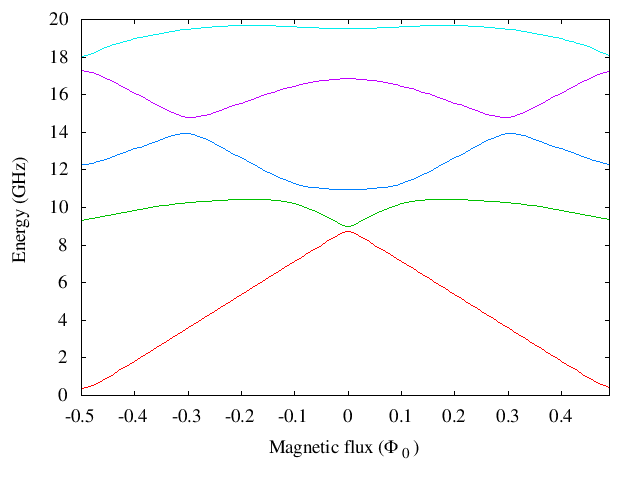
\includegraphics[width=\figwidth]{CPBL-theory.png}
\caption{ Energy spectrum for the CPBL. $E_C=2.5$, $E_J=8.8$, and
  $E_L=0.5$. The y-axis and parameter values are in gigahertz, and the
  x-axis is given in multiples of the base flux, $\phi_0$. (Recall
  that Eqn.~\ref{inner-V} is periodic in $\phi$.)}
\label{cpbl-theory}
\end{figure}

\section{Experimental Data}
Vlad Manucharyan has been measuring the energy spectra of some of the
first CPBL devices ever produced, and one of our immediate goals was
to fit our theoretical spectra against his data. Energy curves were
originally drawn from those data by hand, but a simple threshold
filter automates that process. Raw data (Figs.~\ref{raw-1} and
\ref{raw-2}) can be filtered into sets of points suitable for fitting
(Figs.~\ref{filter-1} and \ref{filter-2}).

\begin{figure} 
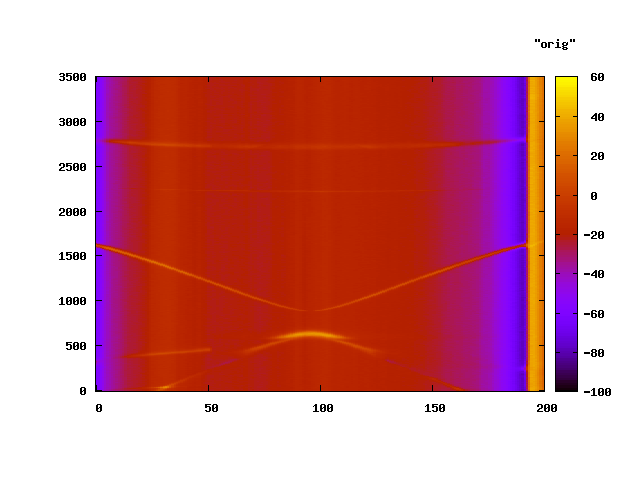
\includegraphics[width=\figwidth]{colorful-data.png}
\caption{ Raw data displayed in Gnuplot. Though the parameters are not
identical, the scale here is approximately a zoom on the central
region of Fig.~\ref{cpbl-theory}}
\label{raw-1}
\end{figure}

\begin{figure}
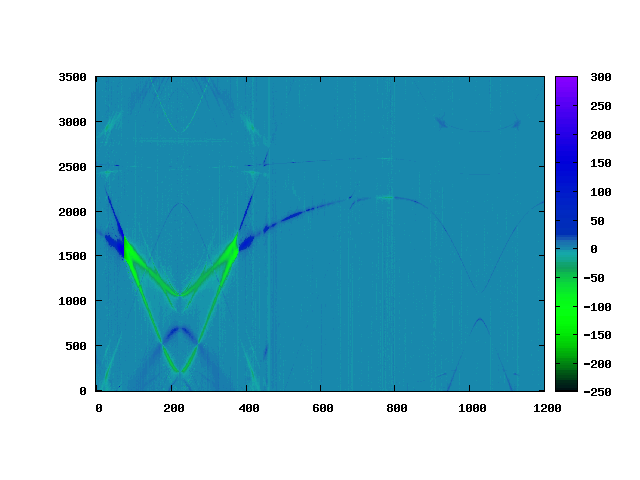
\includegraphics[width=\figwidth]{CPBL-color.png}
\caption{ Raw data displayed in Gnuplot. For scale, the right half of
  this plot is approximately the same area plotted in
  Fig.~\ref{raw-1}. }
\label{raw-2}
\end{figure}

\begin{figure}
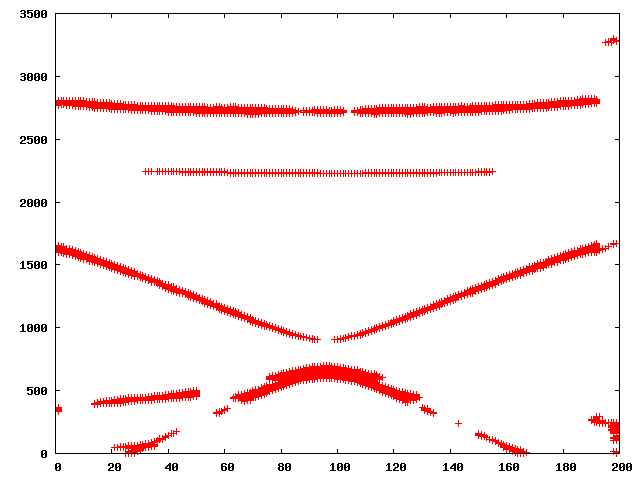
\includegraphics[width=\figwidth]{colorful-points.png}
\caption{ Curves filtered out of the data in Fig.~\ref{raw-1} }
\label{filter-1}
\end{figure}

\begin{figure}
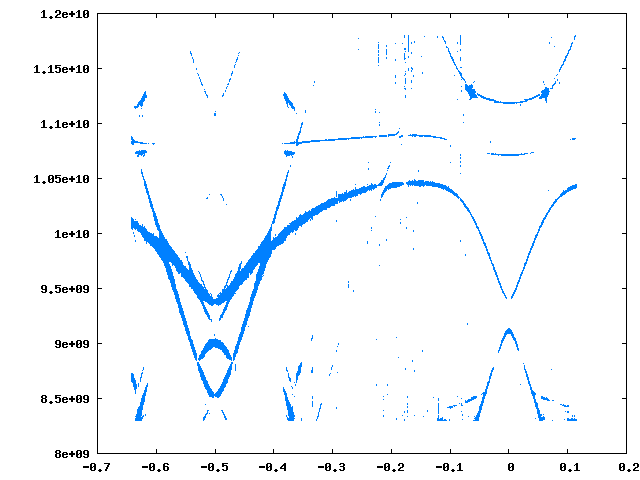
\includegraphics[width=\figwidth]{CPBL-data.png}
\caption{ Curves filtered out of the data in Fig.~\ref{raw-2} }
\label{filter-2}
\end{figure}

There are many ways to define a ``badness of fit'' for theoretical
curves against these data. In our case, the simplest and most
effective method is, for each point in the data set, to find the
vertically nearest curve in the theoretical set, take the difference
between the two, and add together the squares of those differences. We
can then use generic multi-parameter minimization routines to find the
best fitting values of $E_C$, $E_J$, and $E_L$.\cite{Byrd}\cite{Zhu}
The results of this approach are displayed in Figs.~\ref{pre-fit} and
\ref{post-fit}.

\begin{figure}
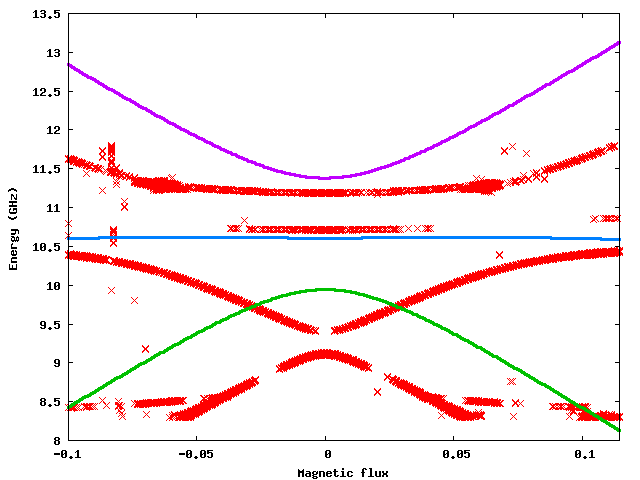
\includegraphics[width=\figwidth]{CPBL-prefit.png}
\caption{ An initial guess for parameter values plotted against
  experimental data from a portion of the set depicted in
  Fig.~\ref{raw-2}. This initial guess is clearly very poor, even
  though none of the parameters is off by more than 20\%.}
\label{pre-fit}
\end{figure}

\begin{figure}
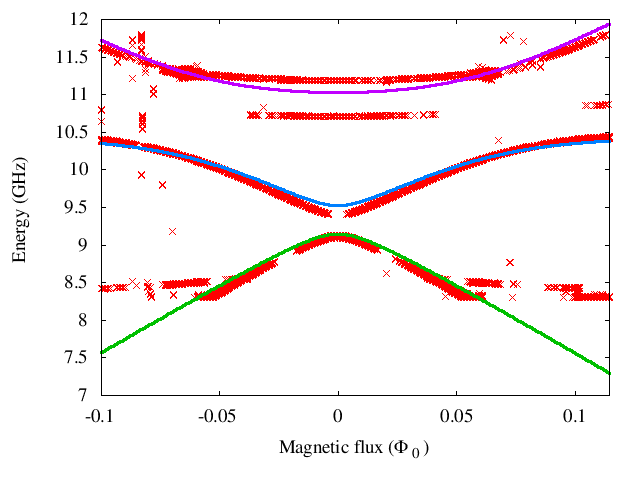
\includegraphics[width=\figwidth]{CPBL-postfit.png}
\caption{ The same data set from Fig.~\ref{pre-fit} after our
  optimization routines adjusted the parameter values from that
  initial guess.}
\label{post-fit}
\end{figure}

The only human input to the fit depicted in Fig.~\ref{post-fit} was
the initial parameter guess and the identification of the zero-flux
point on the x-axis. Note that the lines jutting out to the left and
right of the bottom peak in that figure represent a transition between
two non-ground states, and that a better fit could be had by plotting
those transitions along with the ground state transitions. The line
appearing clearly between the upper two spectral lines in that figure
is not one of these transitions but rather a resonance from our
experimental setup outside the CPBL itself, and it causes the lines
nearest to it to deviate slightly from the theory. Cleaning out these
extraneous points would improve the fit as well, though it would
require more human input.

\section{Speeding it Up}



\section{Conclusion}



\begin{thebibliography}{9}
\bibitem{Byrd} R. H. Byrd, P. Lu, and J. Nocedal. ``A Limited Memory
  Algorithm for Bound Constrained Optimization.'' \textit{SIAM Journal
    on Scientific and Statistical Computing} 16, 5,
  pp. 1190-1208. (1995)
  
\bibitem{Feynman} R. P. Feynman, R. B. Leighton, and
  M. Sands. \textit{The Feynman Lectures on Physics}. Addison-Wesley
  Publishing Company. Vol. 3, Ch. 21-9. (1963)

\bibitem{Vandersypen} L. Vandersypen et al. ``Experimental realization
  of Shor's quantum factoring algorithm using nuclear magnetic
  resonance.'' \textit{Nature} 414, pp. 883-887. (20 December 2001)
  
\bibitem{Zhu} C. Zhu, R. H. Byrd, and J. Nocedal. ``L-BFGS-B, FORTRAN
  routines for large scale bound constrained optimization.''
  \textit{ACM Transactions on Mathematical Software} Vol 23, Num. 4,
  pp. 550 - 560. (1997)

\end{thebibliography}

\end{document}
